\documentclass[aspectratio=169,xcolor=table]{beamer}
\usetheme[style=classic]{mhar-vell}
%\usepackage{helvet}
%*--------------------------------------------------
\usepackage{bibunits}  
%\setbeamertemplate{bibliography item}{[\theenumiv]}
\setbeamertemplate{bibliography item}{\insertbiblabel}
\defaultbibliography{bibliography}
%\defaultbibliographystyle{IEEEtran}
%\defaultbibliographystyle{amsalpha}
\defaultbibliographystyle{abntex2-alf}
%\bibliography{bibliography}
%\usepackage[backend=biber,style=alphabetic,citestyle=authoryear]{biblatex}
% \addbibresource{bibliography.bib}
%\usepackage{natbib}
\usepackage{bibentry}
%*--------------------------------------------------
\usepackage{epigraph}
\usepackage{graphicx}
\usepackage{multirow}
%\usepackage{enumitem}
\usepackage{array}
%\usepackage{multimedia}
\usepackage{media9}
%\usepackage{pdfpc-movie}
\usepackage{tikz}
\usepackage{circledsteps}
\usepackage{listings}
\usepackage[normalem]{ulem}
%\usepackage{Sweave}
%\usepackage{xkeyval}
%\usepackage{palatino}
%\usepackage{pgfpages}
%*--------------------------------------------------
\usepackage[timeinterval=1]{tdclock}
%\usepackage[font=Times,timeinterval=1, timeduration=200,resetatpages=all]{tdclock}
%\usepackage[font=Times,timeinterval=10, timeduration=2.0, timedeath=0, fillcolorwarningsecond=white!60!yellow,timewarningfirst=50,timewarningsecond=80,resetatpages=2]{tdclock}
%*--------------------------------------------------
\usepackage{url}
\usepackage{tabularx,booktabs}
\usepackage{threeparttable}
\usepackage[absolute, overlay]{textpos}
%*--------------------------------------------------
\usepackage{framed, color}
\usepackage[tikz]{bclogo}
\usepackage{spot}
\setspotlightcolor{red!50}
% %\setspotlightstyle{star, fill=red!50}
% %\setspotlightstyle{star points=7}
\usepackage{color,soul}
%\usepackage{xcolor}
\usepackage{tcolorbox}
\usepackage{xcolor}
%*--------------------------------------------------
\usepackage{amsmath}
\usepackage{xfrac}
\usepackage{units}
\usepackage{ulem}
%*-------------------------------------------------------------------------------
%\newcolumntype{C}[1]{>{\centering\arraybackslash}m{#1}}
\newcolumntype{L}[1]{>{\raggedright\let\newline\\\arraybackslash\hspace{0pt}}m{#1}}
\newcolumntype{C}[1]{>{\centering\let\newline\\\arraybackslash\hspace{0pt}}m{#1}}
\newcolumntype{R}[1]{>{\raggedleft\let\newline\\\arraybackslash\hspace{0pt}}m{#1}}
%*-------------------------------------------------------------------------------
%\pgfpagesuselayout{2 on 1}[a4paper,border shrink=5mm]
%\setbeamertemplate{note page}[plain]
%\setbeameroption{show notes on second screen=bottom}
%*-------------------------------------------------------------------------------
\setbeameroption{hide notes}
%\setbeameroption{show only notes}
%\setbeameroption{show notes on second screen=right}
\setbeamertemplate{note page}{\pagecolor{yellow!5}\insertnote}
%*-------------------------------------------------------------------------------
\title              {Estudo Dirigido}
\subtitle           {Kinematic Modeling and Simulation of a SCARA Robot by
Using Solid Dynamics and Verification by MATLAB/Simulink}
\author             {Mateus Seixas}
\email              {mateus\textunderscore seixas@hotmail.com.br}
\advisor            {Orientador: Marco Reis}
\institute          {Robótica e Sistemas Autônomos, Senai Cimatec}
\date               {Outubro de 2021}
% \ulogo        		{Template/logosenaicimatecnegativo}
% \ulogof             {Template/logosenaicimatec2020}
% \ulogoo        		{Template/rosa-logo}
% \ulistelement    	{Template/bullet-white}

%*-------------------------------------------------------------------------------
\graphicspath{{Media/pictures/}}
%*-------------------------------------------------------------------------------
\totalNoSlidesDisabled % To turn off the total number of slides in the footer. Comment this if you want the total number of slides in the footer
%*-------------------------------------------------------------------------------
\begin{document}
%*----------- COVER -------------------------------------------------------------
\begin{frame}[t,plain]
%*----------- sound--------------------------------
    \includemedia[
        width=1ex,
        height=1ex,
        %activate=pageopen, 
        activate=onclick,
        deactivate=onclick,
        %passcontext,
        transparent,
        addresource=./Media/sounds/hip-hop.mp3,
        flashvars={
                    source=./Media/sounds/hip-hop.mp3
                    %&autoPlay=true
                    &autoRewind=true
                    &Play=2s
                    &repeat=always
                    %&Loop=true
        }
    ]
    {}{VPlayer.swf}
%*----------- start-page--------------------------
    \titlepage
%*----------- notes-------------------------------
    \note[item]{Notes can help you to remember important information. Turn on the notes option.}
    \note[item]{Notes can help you to remember important information. Turn on the notes option.}
\end{frame}
%-
%*----------- SECTIONS ----------------------------------------------------------
%*----------- SLIDE -------------------------------------------------------------
\begin{frame}[t]{Artigo de Referência} 
    \begin{center}
        \huge 
        Kinematic Modeling and Simulation of a SCARA Robot by Using Solid Dynamics and Verification by
        MATLAB/Simulink\\
        \!
        \\
        \normalsize
        M. S. Alshamasin, F. Ionescu, R. T. Al-Kasasbeh\\
        2009
        
    \end{center}
\end{frame}
%*----------- SLIDE -------------------------------------------------------------
\begin{frame}[c]{Robôs SCARA}
    \framesubtitle{Selective Compliance Articulated Robot Arm} 
    \begin{columns}
        % \column{.01\textwidth}
        \column{.01\textwidth}
        \column{.5\textwidth}

        \begin{figure}
            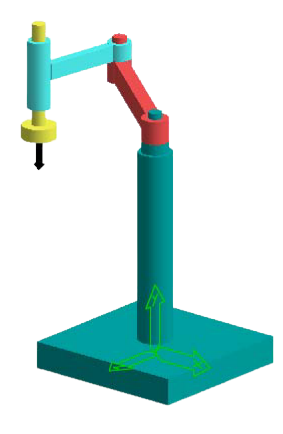
\includegraphics[trim = 0 0 0 0, clip, width=0.7\textwidth]{scara.png}
            %\caption{.}
        \end{figure}

        \column{.49\textwidth}
        \Large
        % São robôs manipuladores que possuem:
        \begin{itemize}
            \item Alta velocidade
            \item Alta precisão
            \item Melhor repetibilidade entre manipuladores
            \item 4 graus de liberdade
        \end{itemize}

    \end{columns}
   
%*----------- notes
    \note[item]{Notes can help you to remember important information. Turn on the notes option.}
\end{frame}
\begin{frame}[c]{Aplicações}

    \begin{columns}
        % \column{.01\textwidth}
        \column{.01\textwidth}
        \column{.49\textwidth}
        \begin{figure}
            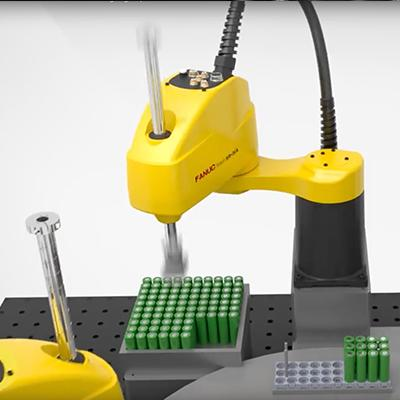
\includegraphics[trim = 0 0 0 0, clip, height=.88\textwidth]{FEA_Speed_assembly-Scara_400x400.jpg}
            %\caption{.}
        \end{figure}    
        % \includemovie{1cm}{1cm}{img07.gif}

        \column{.49\textwidth}
        \begin{figure}
            % 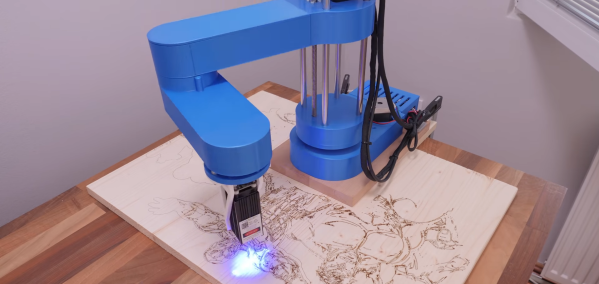
\includegraphics[trim = {5cm 0 5cm 0}, clip, height=.9\textwidth]{2021-08-26-19.png}
            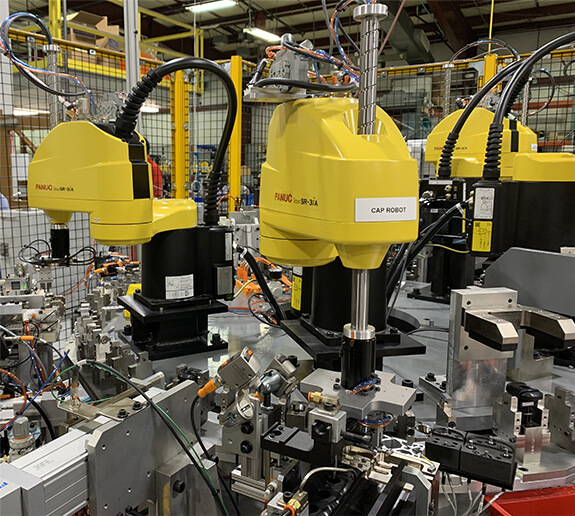
\includegraphics[trim = {0cm 0 0cm 0}, clip, height=.88\textwidth]{aplica2.jpg}
            %\caption{.}
        \end{figure}   
        \column{.01\textwidth}
    
    \end{columns}
    
%*----------- notes
    \note[item]{Notes can help you to remember important information. Turn on the notes option.}
\end{frame}
%*----------- SLIDE -------------------------------------------------------------
\begin{frame}[c]{A Importância das Simulações} 
    % \framesubtitle{Notação Denavit-Hartenberg}
    \begin{columns}
        \column{.01\textwidth}
        \column{.69\textwidth}
        As simulações possuem as seguintes vantagens:
        \begin{itemize}
            \item Fáceis de montar
            \item Baixo custo
            \item Resultados rápido
        \end{itemize}
        Poranto podem ser utilizadas para:
        \begin{itemize}
        \item Prever o comportamento do robô
        \item Programar off-line
        \item Avaliar layout
        \item Fazer estudos de viabilidade
        \item Otimizar o planejamento de trajetória
        \end{itemize}
        \column{.3\textwidth}
        \begin{figure}
            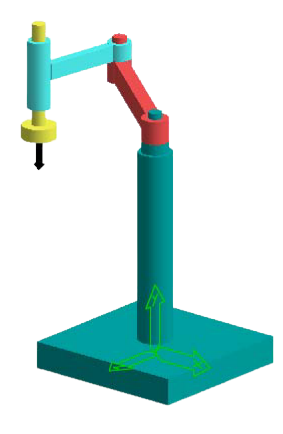
\includegraphics[trim = {0cm 0 0cm 0}, clip, height=1.5\textwidth]{scara2.png}
        \end{figure}   
    
    \end{columns}
    
%*----------- notes
    \note[item]{Tem como objetivo pose do end effector a partir dos deslocamentos angulares e lineares das juntas. Pela notação D-H é possível descrever uma junta com 4 parâmetros.}
\end{frame}
%*----------- SLIDE -------------------------------------------------------------
% \begin{frame}{Graus de Liberdade}
%     \begin{figure}
%         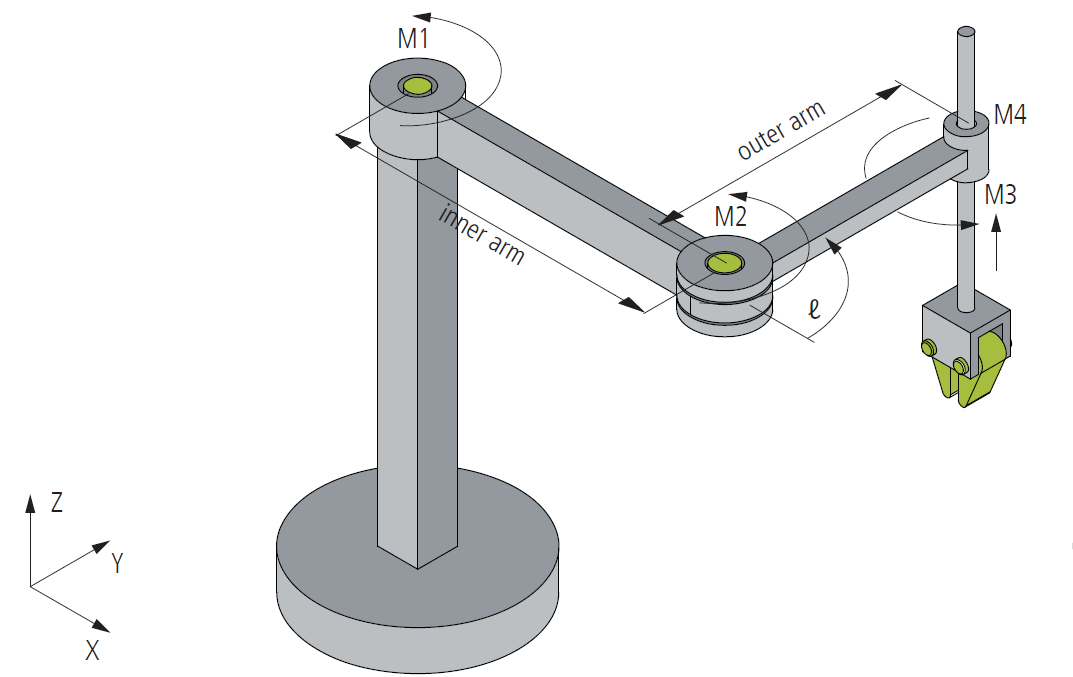
\includegraphics[trim = 160 0 0 0, clip, width=0.6\textwidth]{1232566667__Web.png}
%         %\caption{.}
%     \end{figure}     
% \end{frame}
%*----------- SLIDE -------------------------------------------------------------
\begin{frame}[c]{Cinemática Direta x Cinemática Inversa} 
    % \transdissolve[duration=0.5]

    \begin{figure}
        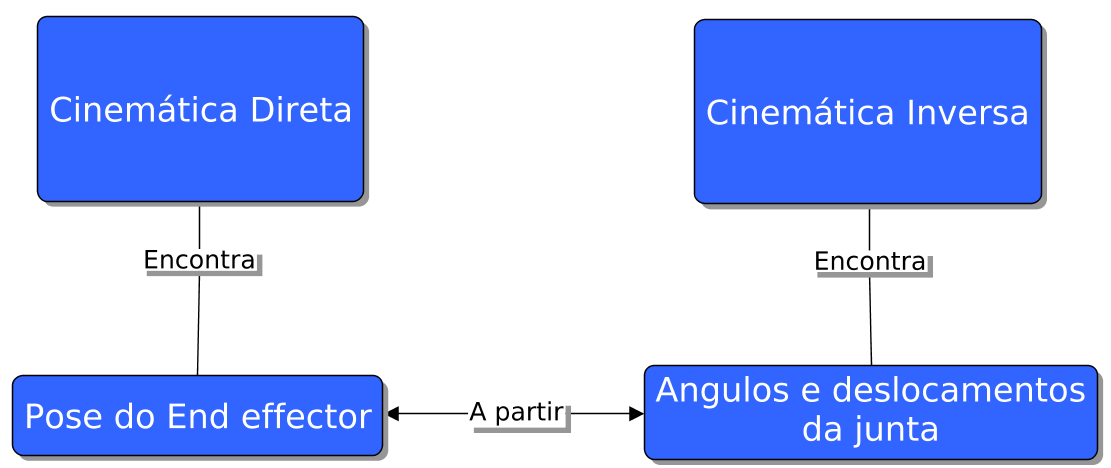
\includegraphics[trim = 0 0 0 0, clip, height=.38\textwidth]{cinematica.png}
        %\caption{.}
    \end{figure}
        
    %*----------- notes
    % \begin{center}
    %     \Wider{%
    %     \begin{shaded}
    %     \begin{center}
    %         \vspace*{0.5cm}
    %         \resizebox{!}{0.7cm}{%
    %             \textcolor{cyan}{G}\textcolor{red}{o}\textcolor{orange}{o}\textcolor{cyan}{g}\textcolor{teal}{l}\textcolor{red}{e}?
    %         }%
    %     \end{center}
    %     \end{shaded}
    %     }%
    % \end{center}
%*----------- notes
    \note[item]{Notes can help you to remember important information. Turn on the notes option.}
\end{frame}
%*----------- SLIDE -------------------------------------------------------------
\begin{frame}[c]{Cinemática Direta} 
    \framesubtitle{Notação Denavit-Hartenberg}
    Tem como objetivo obter o conjunto de equações que descreve a cinemática direta de um robô. \\
    Cada junta do robô é descrita através de 4 parâmetros:
    \begin{itemize}
        \item $\theta$ - Ângulo de rotação da junta
        \item d - Deslocamento da junta
        \item a - Comprimento do elo
        \item $\alpha$ - Ângulo de torção da junta
        
    \end{itemize}

%*----------- notes
    \note[item]{Tem como objetivo pose do end effector a partir dos deslocamentos angulares e lineares das juntas. Pela notação D-H é possível descrever uma junta com 4 parâmetros.}
\end{frame}
%*----------- SLIDE -------------------------------------------------------------
\begin{frame}[c]{Cinemática Direta} 
    \framesubtitle{Notação Denavit-Hartenberg}
    \large
    
    \begin{figure}
        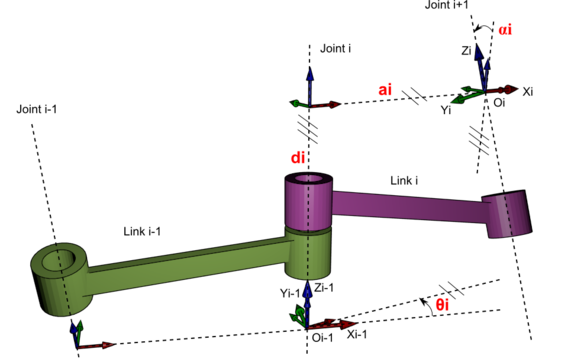
\includegraphics[trim = 0 0 0 0, clip, height=0.4\textwidth]{Classic-DHparameters.png}
    \end{figure}

%*----------- notes
    \note[item]{Tem como objetivo pose do end effector a partir dos deslocamentos angulares e lineares das juntas. Pela notação D-H é possível descrever uma junta com 4 parâmetros.}
\end{frame}
%*----------- SLIDE -------------------------------------------------------------
\begin{frame}[c]{Notação Denavit-Hartenberg} 
    % \framesubtitle{Notação Denavit-Hartenberg}
    \large
    
    \begin{figure}
        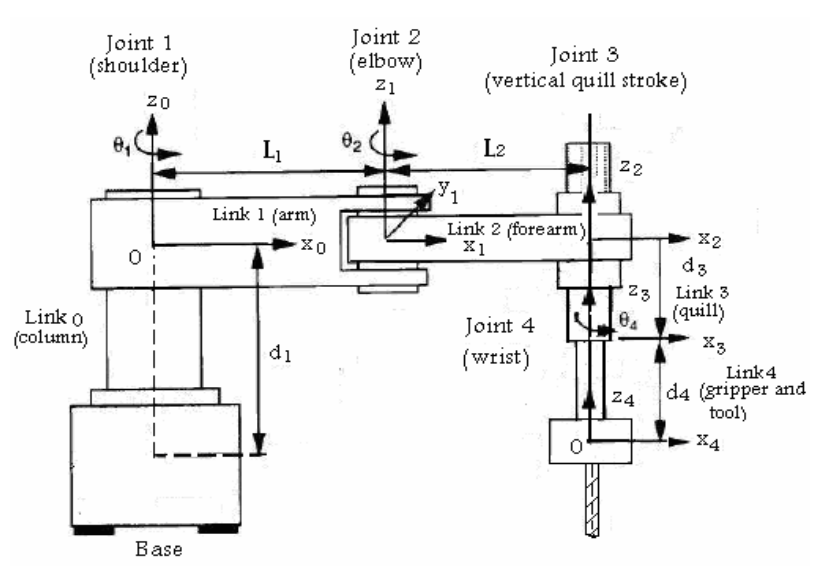
\includegraphics[trim = 0 1cm 0 0, clip, height=0.48\textwidth]{dhnota.png}
    \end{figure}

%*----------- notes
    \note[item]{Tem como objetivo pose do end effector a partir dos deslocamentos angulares e lineares das juntas. Pela notação D-H é possível descrever uma junta com 4 parâmetros.}
\end{frame}
%*----------- SLIDE -------------------------------------------------------------
\begin{frame}[c]{Notação Denavit-Hartenberg} 
    % \framesubtitle{Notação Denavit-Hartenberg}
    \large
    
    \begin{figure}
        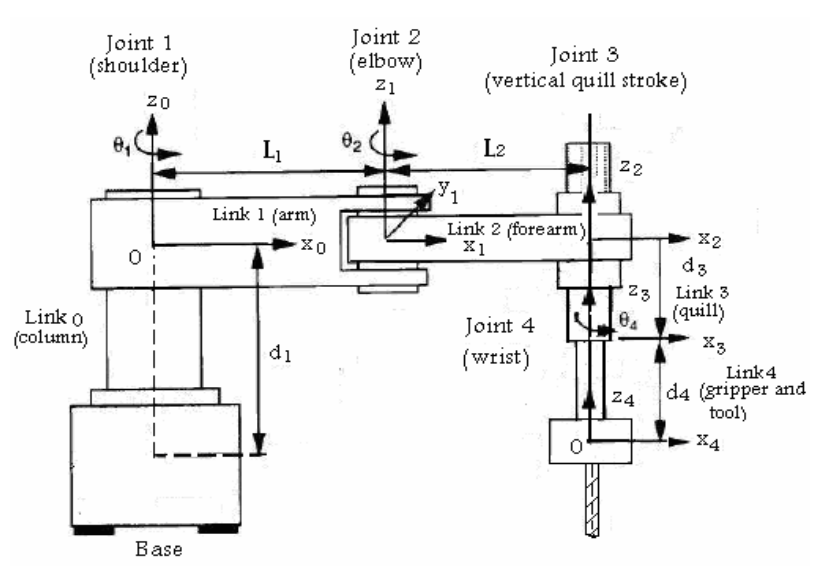
\includegraphics[trim = 0 0 0 0, clip, height=0.35\textwidth]{dhnota.png}
        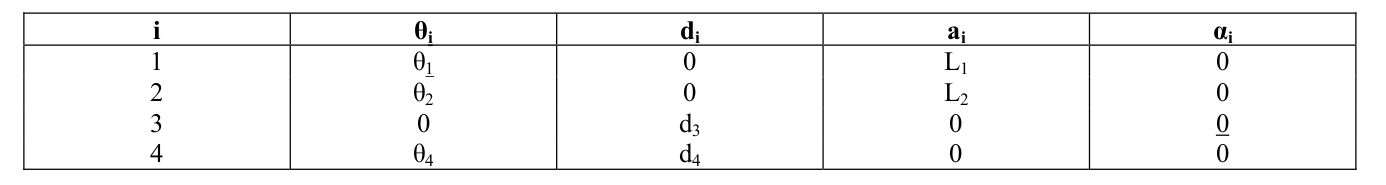
\includegraphics[trim = 0 0 0 0, clip, width=.9\textwidth]{Screenshot from 2021-11-01 18-12-13.png}
    \end{figure}
%*----------- notes
    \note[item]{Tem como objetivo pose do end effector a partir dos deslocamentos angulares e lineares das juntas. Pela notação D-H é possível descrever uma junta com 4 parâmetros.}
\end{frame}
%*----------- SLIDE -------------------------------------------------------------
\begin{frame}[c]{Notação Denavit-Hartenberg} 
    \framesubtitle{Matriz de Transformação Homogênea}
    \large{
    \begin{itemize}
        \item Matriz de transformação da junta (i-1) e i:\\
        \vspace{0.3cm}
        $T_{i}^{i-1}=Rot(z,\theta_{i})\cdot Trans(z,d_{i})\cdot Trans(x,a_{i})\cdot Rot(x,\alpha_{i})$\\
    \end{itemize}
    
    \begin{itemize}
        \item Matriz de transformação homogênea:\\
        \vspace{0.3cm}
        $T_{n}^{0}=T_{1}^{0}\cdot T_{2}^{1} \cdot T_{3}^{2} \cdots T_{n}^{n-1}$
    \end{itemize}
    }
    % 
\includegraphics[clip, trim = 0 0 0 0,  width=.83\textwidth]{databases.jpg}
%*----------- notes
    \note[item]{Tem como objetivo pose do end effector a partir dos deslocamentos angulares e lineares das juntas. Pela notação D-H é possível descrever uma junta com 4 parâmetros.}
\end{frame}
%*----------- SLIDE -------------------------------------------------------------
\begin{frame}[c]{Cinemática Inversa} 
    \large
    % \framesubtitle{Pouco tempo para muito resultado}
    % \transdissolve[duration=0.5]
    A cinemática inversa tem como objetivo encontrar deslocamentos angulares e lineares das juntas a partir da pose do end effector.\\% Normalmente para cada pose existem mais de uma solução.\\
    A matriz de transformação homemogênea é igual ao produto das matrizes de transformação de uma junta para outra:\\
    \vspace{.15cm}

    \begin{center}
        $T_{4}^{0}=T_{1}^{0}\cdot T_{2}^{1} \cdot T_{3}^{2} \cdot T_{4}^{3}$\\
    \end{center}

    \vspace{.15cm}
    Logo, solucionando para a junta 4, por exemplo:\\
    \vspace{.2cm}
    \begin{center}
        $T_{4}^{3}=(T_{3}^{2})^{-1} \cdot (T_{2}^{1})^{-1} \cdot (T_{1}^{0})^{-1} \cdot T_{4}^{0}$    
    \end{center}    
%*----------- notes
    \note[item]{Notes can help you to remember important information. Turn on the notes option.}
\end{frame}
 %*----------- SLIDE -------------------------------------------------------------
 \begin{frame}
    \begin{columns}
        %\column{.01\textwidth}
        \column{0.4\textwidth}
        ~\hfill
            \begin{beamercolorbox}[sep=8em, colsep*=18pt, wd=\textwidth,ht=\paperheight]{title page header}
                \begin{center}
                    \textbf{\huge{DINÂMICA}}\par
                \end{center}
            \end{beamercolorbox}%
            
        \column{.05\textwidth} 
        \column{.6\textwidth}
        \Large
        Para o estudo da dinâmica do robô é necessário modelar:
        \vspace{.4cm}
        \begin{itemize}
            \item Atuadores
            \item Transmissões
            \item Juntas
        \end{itemize}
    \end{columns}
  
%*----------- notes
    \note[item]{Notes can help you to remember important information. Turn on the notes option.}
 \end{frame}
 %*----------- SLIDE -------------------------------------------------------------
\begin{frame}[c]{Resultados} 
    \framesubtitle{$\theta_{1}=1.6493$ rad e $\theta_{2}=1.475-2.6178$ rad}
    \begin{columns}
        \column{0.5\textwidth}
        \begin{center}
            \Large \textbf{Matlab}\\     
        \end{center}
        \begin{figure}
            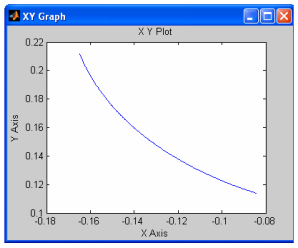
\includegraphics[trim = 0 0 0 0, clip, height=.68\textwidth]{m_1.png}
        \end{figure}
        \column{0.49\textwidth}
        \begin{center}
            \Large \textbf{SD Software}\\    
        \end{center}
        \begin{figure}
            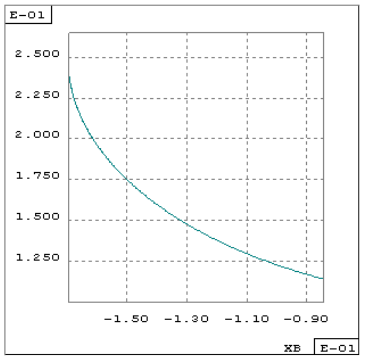
\includegraphics[trim = 0 0 0 0, clip, height=.68\textwidth]{sd_1.png}
        \end{figure}
              
    \end{columns}
\end{frame}
 %*----------- SLIDE -------------------------------------------------------------
 \begin{frame}[c]{Resultados} 
    \framesubtitle{$\theta_{1}=3.0142-0.794125$ rad e $\theta_{2}=2.4495696$ rad}
    \begin{columns}
        \column{0.5\textwidth}
        \begin{center}
            \Large \textbf{Matlab}\\    
        \end{center}
        \begin{figure}
            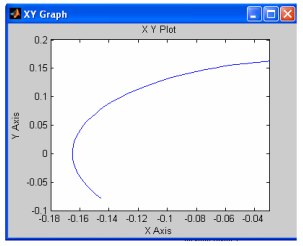
\includegraphics[trim = 0 0 0 0, clip, height=.68\textwidth]{m_2.png}
        \end{figure}
        \column{0.49\textwidth}
        \begin{center}
            \Large \textbf{SD Software}\\   
        \end{center}
        \begin{figure}
            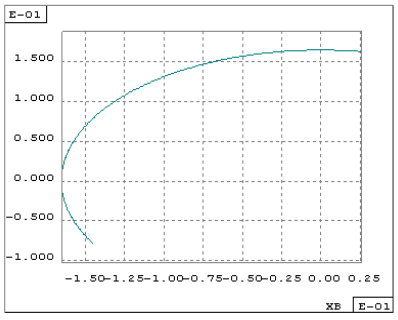
\includegraphics[trim = 0 0 0 0, clip, height=.68\textwidth]{sd_2.png}
        \end{figure}
              
    \end{columns}
\end{frame}
 %*----------- SLIDE -------------------------------------------------------------
 \begin{frame}[c]{Resultados} 
    \framesubtitle{$\theta_{1}=0.232-2.4695$ rad e $\theta_{2}=1.3521- 2.0944$ rad}
    \begin{columns}
        \column{0.5\textwidth}
        \begin{center}
            \Large \textbf{Matlab}\\    
        \end{center}
        \begin{figure}
            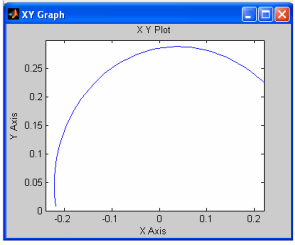
\includegraphics[trim = 0 0 0 0, clip, height=.68\textwidth]{m_3.png}
        \end{figure}
        \column{0.49\textwidth}
        \begin{center}
            \Large \textbf{SD Software}\\    
        \end{center}
        \begin{figure}
            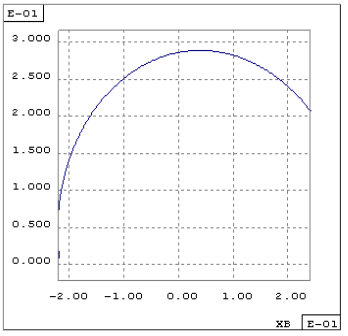
\includegraphics[trim = 0 0 0 0, clip, height=.68\textwidth]{sd_3.png}
        \end{figure}
              
    \end{columns}
\end{frame}
%*----------- SLIDE -------------------------------------------------------------
\begin{frame}[c]{Conclusão} 
\Large
\begin{itemize}
    \item Foi desenvolvido um completo modelo matemático
    \item As equações de cinemática direta e inversa foram obtidas através da notação de Danevit-Hartenberg
    \item Foram feitas simulações em Matlab e Solid Dynamics Software
    \item Os resultados de ambos softwares foram concordantes
\end{itemize}
\end{frame}

% \begin{frame}[c]{teste}
%     \begin{center}
%         \Wider{%
%         \begin{shaded}
%         \begin{center}
%             \vspace*{0.5cm}
%             \resizebox{!}{5cm}{%
%             \begin{figure}
%                 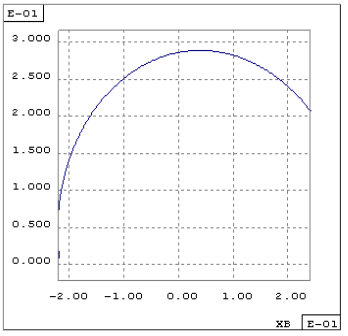
\includegraphics[trim = 0 0 0 0, clip, height=1\textwidth]{sd_3.png}
%             \end{figure}    
%             % \textcolor{cyan}{G}\textcolor{red}{o}\textcolor{orange}{o}\textcolor{cyan}{g}\textcolor{teal}{l}\textcolor{red}{e}?
%             }%
%         \end{center}
%         \end{shaded}
%         }%
%     \end{center}
% \end{frame}[c]{teste}


%*----------- SLIDE -------------------------------------------------------------
\begin{frame}[t]{Melhoria na busca de artigos}
    \framesubtitle{Existe algum método eficiente?}
    %\transboxin[duration=1,direction=30]
    A biblioteconomia.

    \begin{figure}
        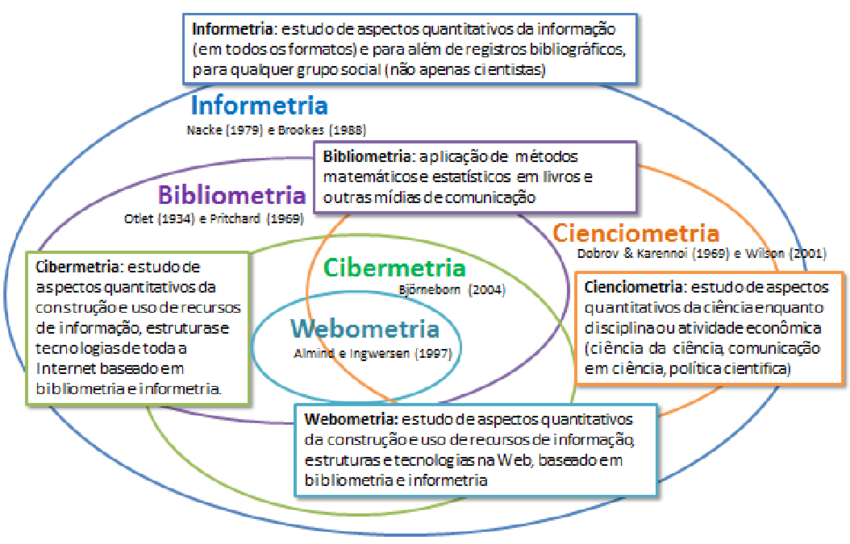
\includegraphics[trim = 0 0 0 0, clip, width=0.6\textwidth]{biblioeconomia.png}
        %\caption{.}
    \end{figure}
%*----------- notes
    \note[item]{Notes can help you to remember important information. Turn on the notes option.}
\end{frame}
%-
%*----------- SLIDE -------------------------------------------------------------
\begin{frame}[t]{Bibliometria}
    \begin{itemize}
        \item É um campo da biblioteconomia e da ciência da informação.
        \item Aplica métodos estatísticos e matemáticos para analisar e construir indicadores sobre a dinâmica e evolução da informação científica e tecnológica.
        \item Medir o impacto das publicações e dos serviços de disseminação da informação.
        \item Identificar autores e instituições mais produtivas.
        \item Todos os estudos que tentam quantificar os processos de comunicação escrita. \cite{pritchard1969statistical}
        \item Avaliar a produção científica. \cite{costa2020ciencia}
        \item Estudar relações entre a ciência e a tecnologia. \cite{maricato2010dinamica}
    \end{itemize}

    \begin{figure}
        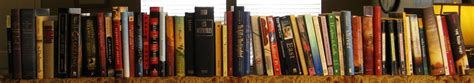
\includegraphics[trim = 0 0 0 0, clip, width=0.7\textwidth]{books-banner.jpeg}
        %\caption{.}
    \end{figure}
   
    % \begin{columns}[t]
    %     \column{.45\textwidth}
    %         detalhar sistemas em subconjuntos\\
    %         listar possíveis modos de falhas\\
    %         analisar cada modo de falha, juntamente com suas possíveis causas e sintomas
    %     \column{.45\textwidth}
    %         estimar os efeitos de cada modo de falhas\\
    %         estimar a criticidade de cada efeito\\
    %         identificar ações para minimizar falhas
    % \end{columns}
%*----------- notes
    \note[item]{Notes can help you to remember important information. Turn on the notes option.}
\end{frame}
%-
%*----------- SLIDE -------------------------------------------------------------
\begin{frame}[t]{Principais autores}
    %\framesubtitle{Lei de Bradford}
    % \begin{figure}
    %     %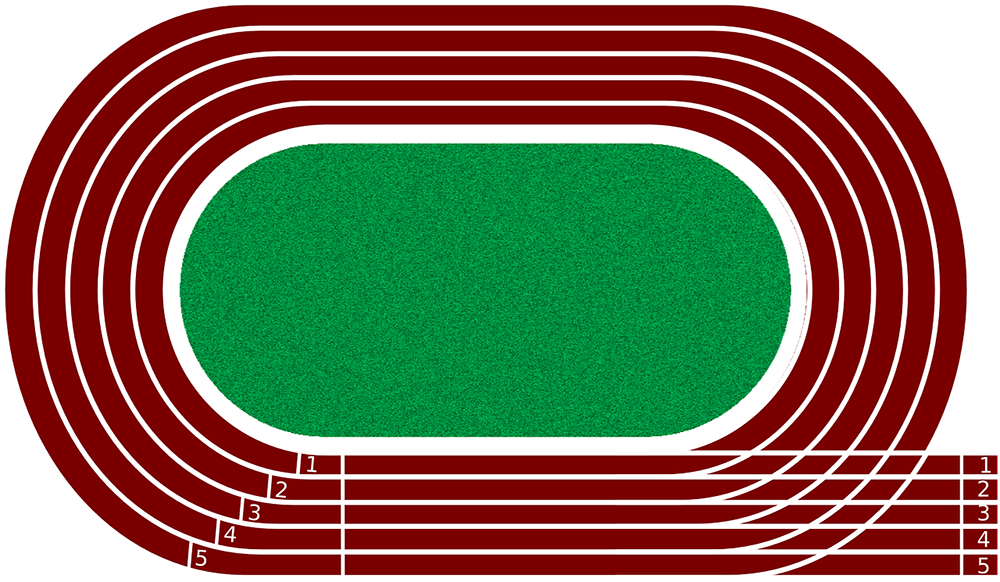
\includegraphics[width=0.7\textwidth]{pista_corrida}
       
    %     \roundpic[xshift=0cm,yshift=0cm]{3cm}{7cm}{pista_corrida}
          
    %     \caption{Formato de um pista de corrida.\cite{agostini2007}}
    % \end{figure}

    \begin{columns}
        %\column{.01\textwidth}
        \column{.33\textwidth}
            \centering
            \roundpic[xshift=0cm,yshift=-0.5cm]{5cm}{7cm}{Samuel_Clemente_Bradford}
            Samuel Clement Bradford\\
            1934
        \column{.33\textwidth}
            \centering
            \roundpic[xshift=0cm,yshift=0cm]{5cm}{7cm}{Alfredo-Lotka}
            Alfred James Lotka\\
            1926
        \column{.33\textwidth}
            \centering
            \roundpic[xshift=0cm,yshift=-1cm]{5cm}{7cm}{George-Zipf}
            George Kingsley Zipf\\
            1940
    \end{columns}

%*----------- notes
    \note[item]{Notes can help you to remember important information. Turn on the notes option.}
\end{frame}
%-
%*----------- SLIDE -------------------------------------------------------------
\begin{frame}[t]{As principais leis bibliométricas}
    \framesubtitle{Lei de Bradford}
    % \begin{figure}
    %     %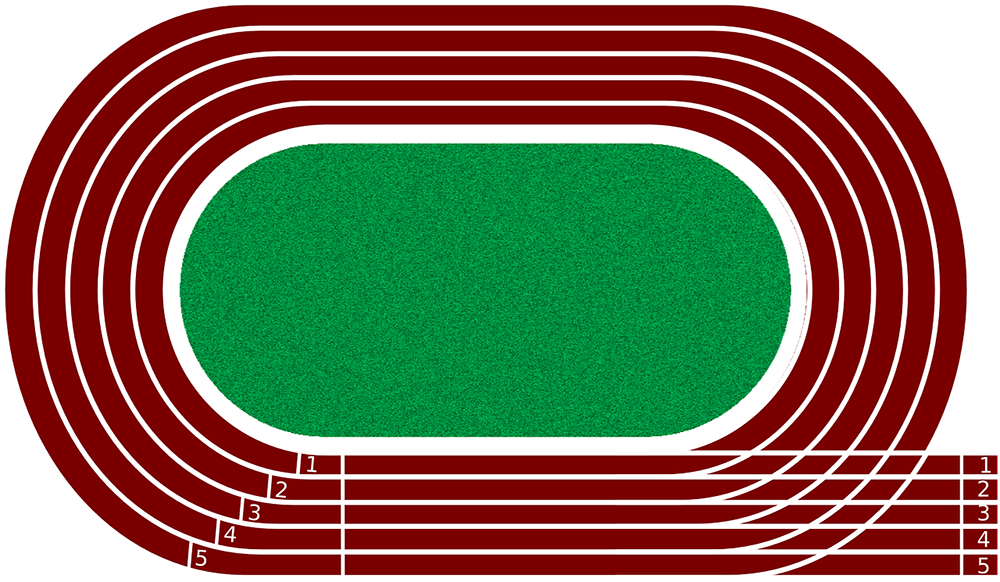
\includegraphics[width=0.7\textwidth]{pista_corrida}
       
    %     \roundpic[xshift=0cm,yshift=0cm]{3cm}{7cm}{pista_corrida}
          
    %     \caption{Formato de um pista de corrida.\cite{agostini2007}}
    % \end{figure}

    \begin{columns}
        \column{.1\textwidth}
        \column{.3\textwidth}

        \begin{figure}
            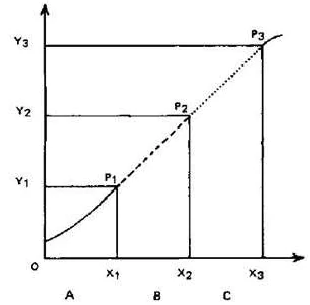
\includegraphics[trim = 0 0 0 0, clip, width=0.7\textwidth]{bradford-2.png}
            %\caption{.}
        \end{figure}

        \centering
        $F(x) = a + b \log x$
        \column{.69\textwidth}
        A lei de Bradford objetiva conhecer o núcleo de periódicos produzidos em determinado tema.\\
        \scriptsize{
            Bradford realiza uma série de estudos que culminam, em 1934, com a formulação da \textbf{lei da dispersão}.\\
            O autor percebe que, numa coleção de periódicos sobre geofísica, existe sempre um núcleo menor de periódicos relacionados de maneira estreita, sendo que o número de perióidocs em cad zona aumenta, enquanto a produtividade diminui.\\
            Analisando 326 períodicos, ele descobriu que 9 periódicos continham 429 artigos, 59 continham 499 e 258 continham 404 artigos.
        }
    \end{columns}

    \vspace*{0.2cm}
    \begin{itemize}
        \item Medir produtividade dos periódicos
        \item Estabelecer núcleo e as áreas de dispersão 
        \item Permite fazer a estimativa do grau de relevância das revistas de conhecimentos
    \end{itemize}
%*----------- notes
    \note[item]{Notes can help you to remember important information. Turn on the notes option.}
\end{frame}
%-
%*----------- SLIDE -------------------------------------------------------------
\begin{frame}[t]{As principais leis bibliométricas}
    \framesubtitle{Lei de Lotka}
    % \begin{figure}
    %     %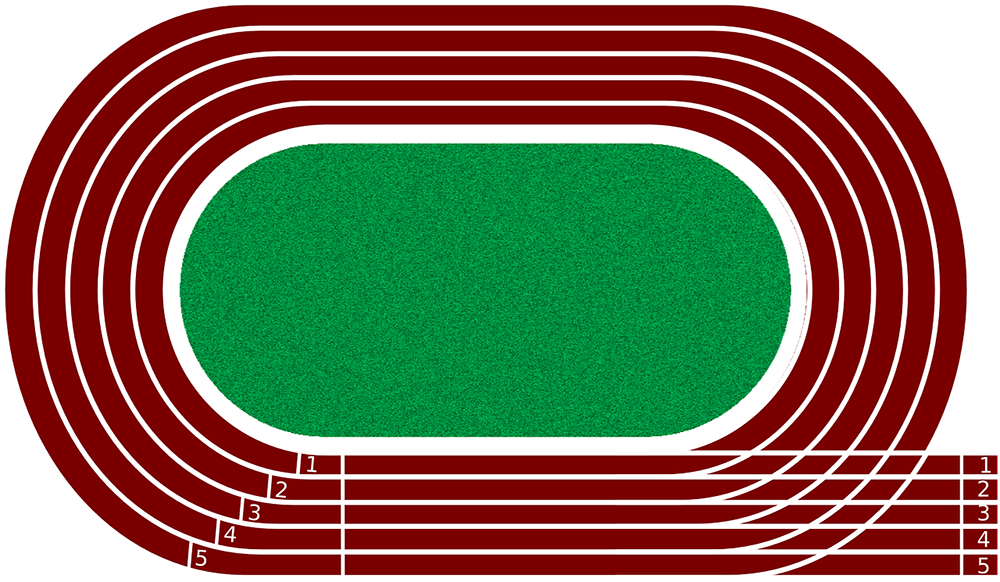
\includegraphics[width=0.7\textwidth]{pista_corrida}
       
    %     \roundpic[xshift=0cm,yshift=0cm]{3cm}{7cm}{pista_corrida}
          
    %     \caption{Formato de um pista de corrida.\cite{agostini2007}}
    % \end{figure}

    \begin{columns}
        \column{.01\textwidth}
        \column{.5\textwidth}

        \begin{figure}
            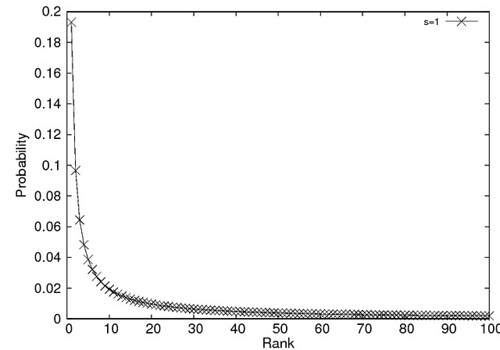
\includegraphics[trim = 0 0 0 0, clip, width=0.6\textwidth]{lotka}
            %\caption{.}
        \end{figure}

        \centering
        $Y = \frac{C}{X^n}$\\
        $Y$ \scriptsize{é a frequência relativa de autores com $X$ publicações.}\\
        $C$ \scriptsize{é a constante que depende da área $X$ é o número de publicações.}

        \column{.49\textwidth}
        A lei de Lotka visa definir as maiores contribuições de pesquisadores em determinadas áreas do conhecimento.\\
        %\scriptsize{
            Lotka descobriu que uma larga proporção da literatura científica é produzida por um pequeno número de autores, e um grande número de pequenos produtores se iguala, em produção, ao reduzido número de grandes produtores.
        %}
    \end{columns}

    \vspace*{0.2cm}

%*----------- notes
    \note[item]{Notes can help you to remember important information. Turn on the notes option.}
\end{frame}
%-
%*----------- SLIDE -------------------------------------------------------------
\begin{frame}[t]{As principais leis bibliométricas}
    \framesubtitle{Lei de Zipf}
    % \begin{figure}
    %     %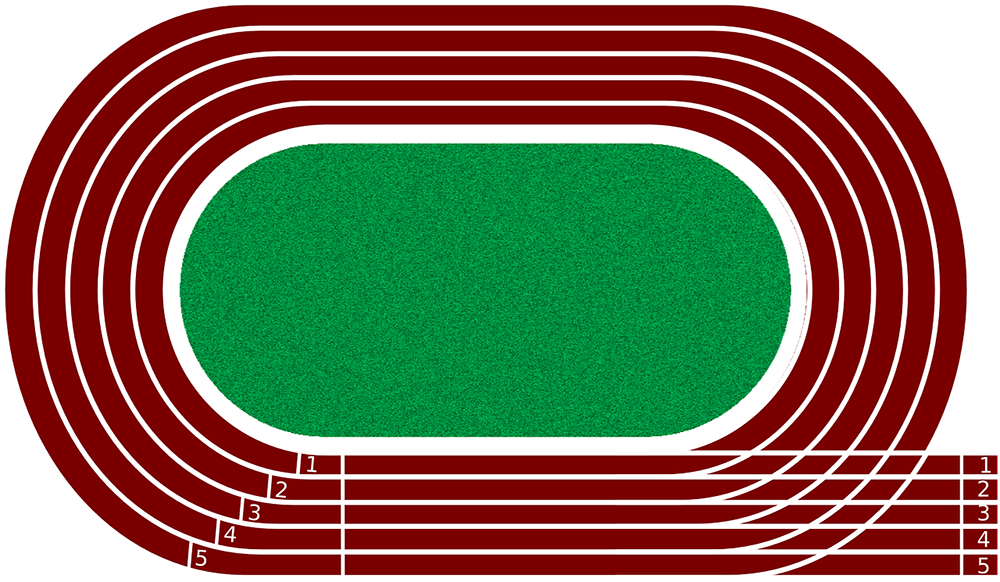
\includegraphics[width=0.7\textwidth]{pista_corrida}
       
    %     \roundpic[xshift=0cm,yshift=0cm]{3cm}{7cm}{pista_corrida}
          
    %     \caption{Formato de um pista de corrida.\cite{agostini2007}}
    % \end{figure}

    \begin{columns}
        \column{.01\textwidth}
        \column{.5\textwidth}

        \begin{figure}
            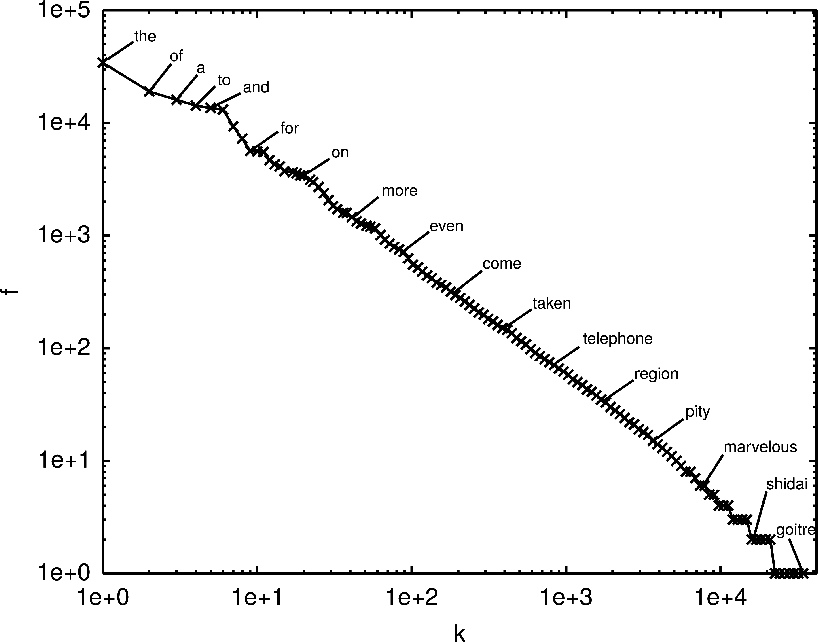
\includegraphics[trim = 0 0 0 0, clip, width=0.5\textwidth]{Figura-1-Lei-de-Zipf-no-Ingles-escrito-dados-do-OANC-Rank-k-versus-frequencia-de.png}
            %\caption{.}
        \end{figure}

        \centering
        $f(n) = \frac{K}{n}$\\
        $f(n)$ \scriptsize{é a frequência de ocorrência de uma palavra}\\
        $n$ \scriptsize{é a ordem de frequência}
        $K$ \scriptsize{é a constante}\\

        \column{.49\textwidth}
        A lei de Zipf pontua a frequência com que certas palavras aparecem nos textos científicos de maneira a definir sua representatividade neste contexto.\\
        \scriptsize{
            Diante desta visão, Zipf formulou o \textbf{princípio do menor esforço}: existe uma economia do uso de palavras, e se a tendência é usar o mínimo significa que elas não vão se dispersar, pelo contrário, uma mesma palavra vais ser usada muitas vezes; as palavras mais usadas indicam o assunto do documento.
        }
    \end{columns}

    \vspace*{0.2cm}
    \begin{itemize}
        \item Trata e mede a frequência de ocorrência de palavras em vários textos.
        \item As palavras mais usadas indicam o assunto.
    \end{itemize}
%*----------- notes
    \note[item]{Notes can help you to remember important information. Turn on the notes option.}
\end{frame}
%-
%*----------- SLIDE -------------------------------------------------------------
\begin{frame}[t]{O fator de impacto}
    %\transboxin[duration=1,direction=30]
    \large{Medida que reflete o número médio de citações de artigos científicos publicados.}\\

    \vspace*{0.2cm}
	Tem como objetivo avaliar a importância de um dado periódico em sua área.

    \begin{figure}
        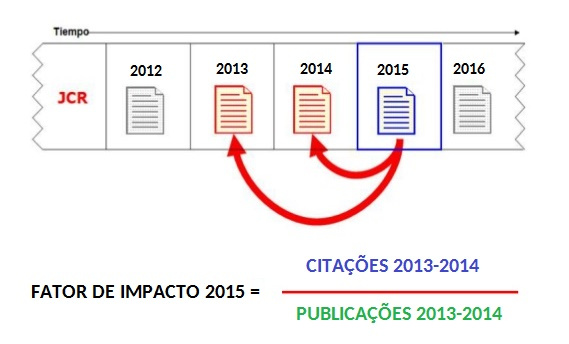
\includegraphics[trim = 0 0 0 0, clip, width=0.6\textwidth]{fi.jpg}
        %\caption{.}
    \end{figure}
%*----------- notes
    \note[item]{Notes can help you to remember important information. Turn on the notes option.}
\end{frame}
%-
%*----------- SLIDE -------------------------------------------------------------
\begin{frame}{Principais estudos da Bibliometria}
    % \begin{table}[ht!]
    %     \centering
    %         \caption{PERCENTUAL DE CONCLUSÃO POR EQUIPE}
    %         \begin{tabular}{|l|c|c|c|c|} \hline
    %             \textbf{EQUIPE}&\textbf{04/05}&\textbf{11/05}&\textbf{18/05}&\textbf{25/05}\\ \hline
    %             RAJA & 17\% &32\% & &  \\ \hline
    %             BORG & 0\% &41\% & &  \\ \hline
    %             TIMON-HM & 5\% &47\% & &  \\ \hline
    %         \end{tabular}
    % \end{table}

	\begin{table}[ht!]
		%\scalefont{0.7}
        \resizebox{0.9\textwidth}{!}{
		\begin{tabular}{|l|c|l|}
            \hline
            \multicolumn{1}{|c|}{\textbf{Leis e Princípios}} & \textbf{Foco de Estudo} & \multicolumn{1}{c|}{\textbf{Principais Aplicações}}                                                                         \\ \hline
            Lei de Bradford                                  & periódicos               & \begin{tabular}[c]{@{}l@{}}estimar o grau de relevância de periódicos\end{tabular}         \\ \hline
            Lei de Lotka                                     & autores                  & \begin{tabular}[c]{@{}l@{}}estimar o grau de relevância de autores\end{tabular}            \\ \hline
            Leis de Zipf                                     & palavras                 & \begin{tabular}[c]{@{}l@{}}indexação automática de artigos científicos\\ e tecnológicos\end{tabular}                        \\ \hline
            Fator de Impacto               & citações                 & \begin{tabular}[c]{@{}l@{}}estimar o grau de relevância de artigos, \\ cientistas e periódicos científicos\end{tabular} \\ \hline
            Acoplamento Bibliográfico                        & citações                 & \begin{tabular}[c]{@{}l@{}}estimar o grau de ligação de dois ou mais \\ artigos\end{tabular}                                \\ \hline
            Co-citação                                       & citações                 & \begin{tabular}[c]{@{}l@{}}estimar o grau de ligação de dois ou mais \\ artigos\end{tabular}                                \\ \hline
            Obsolescência da Literatura                      & citações                 & \begin{tabular}[c]{@{}l@{}}estimar o declínio da literatura de \\ determinada área do conhecimento\end{tabular}             \\ \hline
            Vida-média                                       & citações                 & \begin{tabular}[c]{@{}l@{}}estimar a vida-média de uma unidade da\\  literatura de dada área do conhecimento\end{tabular}   \\ \hline
		\end{tabular}
        }
	\end{table}

%*----------- notes
\note[item]{Notes can help you to remember important information. Turn on the notes option.}
\end{frame}
%-
%*----------- SLIDE -------------------------------------------------------------
\begin{frame}[c]{}

    \centering
    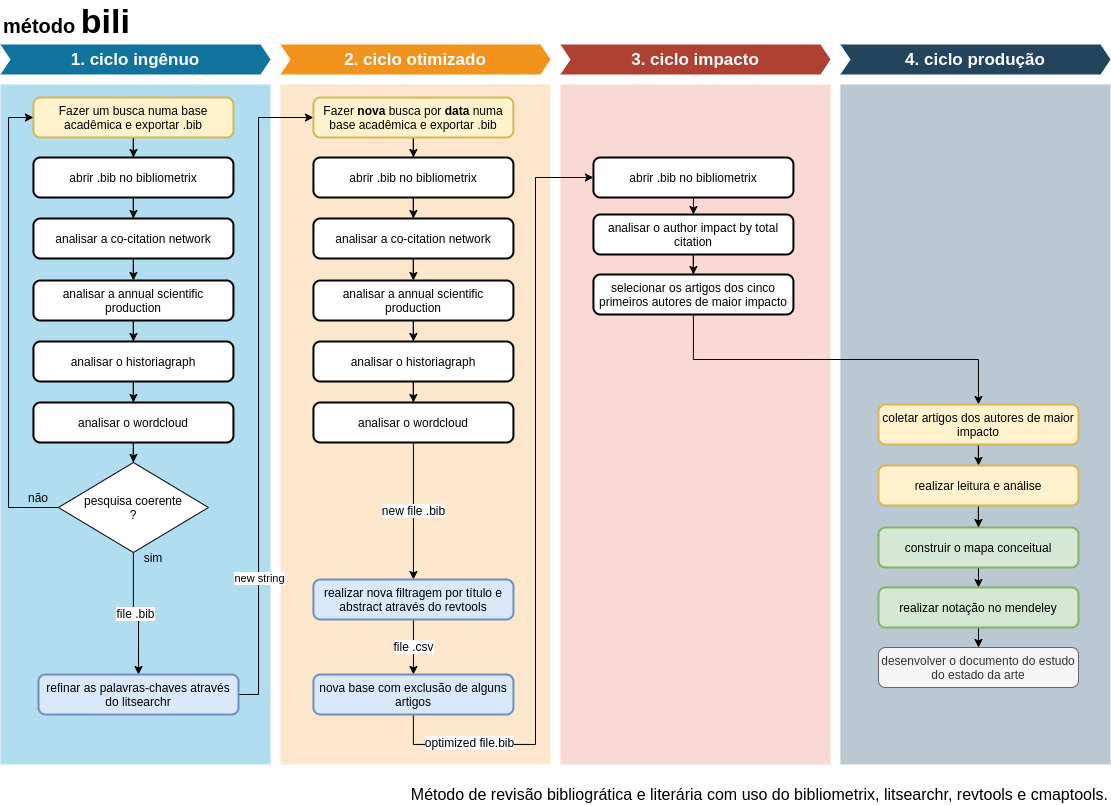
\includegraphics[width=.85\textwidth, trim= 0 30 0 0, clip]{revisão bibliogrática Diagram.png}
    
        
    % \begin{tikzpicture}[remember picture,overlay]
    %     \draw[red,very thick] (cmark) circle[x radius=8mm,y radius=4mm]; 
    % \end{tikzpicture}
%*----------- notes
    \note[item]{Notes can help you to remember important information. Turn on the notes option.}
\end{frame}
%-
%*----------- SLIDE -------------------------------------------------------------
\begin{frame}[t]{O progresso das equipes}
    Um dos indicadores para o acompanhamento das equipes será o percentual de conclusão geral da equipe.
    O planejamento das atividades deverá seguir a metodologia aplicada no desenvolvimento de projetos de robótica.
    \newline
    %\vspace{0.5cm}
    \begin{table}[ht!]
    \centering
        \caption{PERCENTUAL DE CONCLUSÃO POR EQUIPE}
        \begin{tabular}{|l|c|c|c|c|} \hline
            \textbf{EQUIPE}&\textbf{04/05}&\textbf{11/05}&\textbf{18/05}&\textbf{25/05}\\ \hline
            RAJA & 17\% &32\% & &  \\ \hline
            BORG & 0\% &41\% & &  \\ \hline
            TIMON-HM & 5\% &47\% & &  \\ \hline
        \end{tabular}
    \end{table}
%*----------- notes
    \note[item]{Notes can help you to remember important information. Turn on the notes option.}
\end{frame}
%-
%*----------- SLIDE -------------------------------------------------------------
\begin{frame}[t]{Finalização}
    \begin{itemize}
        \item Cada líder deverá realizar a apresentação final do desafio no dia 25/maio/2020.
        \item No dia da apresentação, somente o líder poderá responder os questionamentos emitidos pelos facilitadores.
        \item A avaliação será da equipe, não havendo avaliação individual dos integrantes da equipe com exceção do líder de cada equipe.
        \item A apresentação deverá ser desenvolvida em latex.
        \item Os videos dos desafios deverão estar contidos na apresentação final.
        \item Os videos deverão ser completos, tendo começo, meio e fim da missão realizada.
    \end{itemize}
%*----------- notes
    \note[item]{Notes can help you to remember important information. Turn on the notes option.}
\end{frame}
%-
%*----------- SLIDE -------------------------------------------------------------
\begin{frame}[c]{A importância atual da robótica}
    \begin{center}
        % \movie[loop,width=0.6\linewidth,height=0.3375\linewidth,showcontrols=false,autostart]{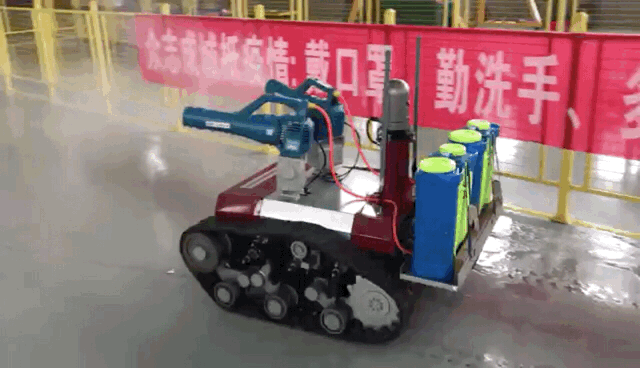
\includegraphics[width=0.6\textwidth]{Media/gifs/robotdesinfec0.png}}{Media/gifs/robotdesinfec.wmv}
    
        \includemedia[
            width=0.7\linewidth,
            totalheight=0.39375\linewidth,
            activate=pageopen,
            passcontext, 
            %transparent,
            addresource=./Media/gifs/robotdesinfec.wmv,
            flashvars={
            source=./Media/gifs/robotdesinfec.wmv
            &autoPlay=true
            &autoRewind=true
            &loop=true}
            ]{\fbox{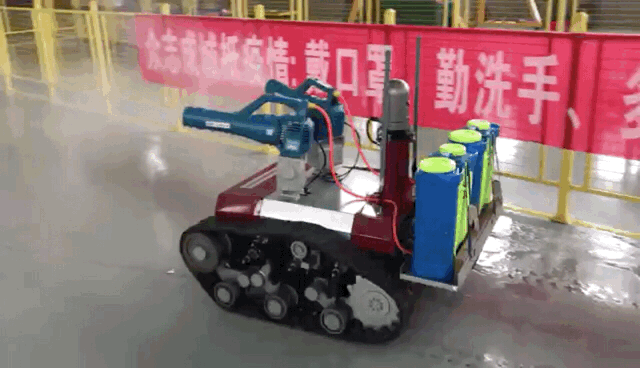
\includegraphics{Media/gifs/robotdesinfec0.png}}}{VPlayer.swf}
    \end{center}
%  %\movie[width=8cm,height=4.5cm]{test}{../Movies/Darwin-OP.mp4}

% % \includemedia[
% %     width=0.4\linewidth,
% %     totalheight=0.225\linewidth,
% %     activate=pageopen,
% %     passcontext,  %show VPlayer's right-click menu
% %     addresource=../Movies/Darwin-OP.mp4,
% %     flashvars={
% %       %important: same path as in `addresource'
% %       source=../Movies/Darwin-OP.mp4
% %     }
% %   ]{\fbox{Click!}}{VPlayer.swf}

%     \pdfpcmovie{\includegraphics[width=\textwidth]{Darwin-OP}}{Darwin-OP.mp4}

%*----------- notes
    \note[item]{Notes can help you to remember important information. Turn on the notes option.}
 \end{frame}
%-
%*----------- SLIDE -------------------------------------------------------------
\begin{frame}[fragile]{A importância atual da robótica}
    Para a implentação de R gráficos deve-se realizar os seguintes comando no ambiente R:

    \begin{lstlisting}[language=R]
        library(tikzDevice)
        beamer.parms = list(paperwidth   = 364.19536/72,
                    paperheight  = 273.14662/72,
                    textwidth    = 307.28987/72,
                    textheight   = 269.14662/72)
        tikz("./your_file.tex", 
            width = beamer.parms$textwidth, 
            height = beamer.parms$textheight)
        ggqqplot(na.omit(my_data$col2))
        dev.off()
    \end{lstlisting}

    \begin{columns}
        \column{.01\textwidth}
        \column{.59\textwidth}
            \textbf{A penúltima linha do texto acima é o códifo em R para a construção do gráfico.}
                
        \column{.4\textwidth}
            \centering
            \begin{tikzpicture}[thick, scale=0.4, every node/.style={scale=0.1}]
                \node[at=(current page.center)] {
               %% Created by tikzDevice version 0.12.3 on 2020-05-14 20:48:40
% !TEX encoding = UTF-8 Unicode
\begin{tikzpicture}[x=1pt,y=1pt]
\definecolor{fillColor}{RGB}{255,255,255}
\path[use as bounding box,fill=fillColor,fill opacity=0.00] (0,0) rectangle (308.44,270.16);
\begin{scope}
\path[clip] (  0.00,  0.00) rectangle (308.44,270.16);
\definecolor{drawColor}{RGB}{255,255,255}
\definecolor{fillColor}{RGB}{255,255,255}

\path[draw=drawColor,line width= 0.6pt,line join=round,line cap=round,fill=fillColor] (  0.00,  0.00) rectangle (308.44,270.16);
\end{scope}
\begin{scope}
\path[clip] ( 36.99, 35.59) rectangle (302.44,264.16);
\definecolor{fillColor}{RGB}{255,255,255}

\path[fill=fillColor] ( 36.99, 35.59) rectangle (302.44,264.16);
\definecolor{drawColor}{RGB}{0,0,0}
\definecolor{fillColor}{RGB}{0,0,0}

\path[draw=drawColor,line width= 0.4pt,line join=round,line cap=round,fill=fillColor] ( 49.06, 83.70) circle (  1.96);

\path[draw=drawColor,line width= 0.4pt,line join=round,line cap=round,fill=fillColor] ( 78.84, 92.35) circle (  1.96);

\path[draw=drawColor,line width= 0.4pt,line join=round,line cap=round,fill=fillColor] ( 95.19,107.92) circle (  1.96);

\path[draw=drawColor,line width= 0.4pt,line join=round,line cap=round,fill=fillColor] (107.25,111.38) circle (  1.96);

\path[draw=drawColor,line width= 0.4pt,line join=round,line cap=round,fill=fillColor] (117.17,121.76) circle (  1.96);

\path[draw=drawColor,line width= 0.4pt,line join=round,line cap=round,fill=fillColor] (125.79,125.22) circle (  1.96);

\path[draw=drawColor,line width= 0.4pt,line join=round,line cap=round,fill=fillColor] (133.57,128.68) circle (  1.96);

\path[draw=drawColor,line width= 0.4pt,line join=round,line cap=round,fill=fillColor] (140.76,132.14) circle (  1.96);

\path[draw=drawColor,line width= 0.4pt,line join=round,line cap=round,fill=fillColor] (147.56,133.87) circle (  1.96);

\path[draw=drawColor,line width= 0.4pt,line join=round,line cap=round,fill=fillColor] (154.07,137.33) circle (  1.96);

\path[draw=drawColor,line width= 0.4pt,line join=round,line cap=round,fill=fillColor] (160.40,142.52) circle (  1.96);

\path[draw=drawColor,line width= 0.4pt,line join=round,line cap=round,fill=fillColor] (166.62,142.52) circle (  1.96);

\path[draw=drawColor,line width= 0.4pt,line join=round,line cap=round,fill=fillColor] (172.81,145.98) circle (  1.96);

\path[draw=drawColor,line width= 0.4pt,line join=round,line cap=round,fill=fillColor] (179.04,149.44) circle (  1.96);

\path[draw=drawColor,line width= 0.4pt,line join=round,line cap=round,fill=fillColor] (185.37,159.82) circle (  1.96);

\path[draw=drawColor,line width= 0.4pt,line join=round,line cap=round,fill=fillColor] (191.88,161.55) circle (  1.96);

\path[draw=drawColor,line width= 0.4pt,line join=round,line cap=round,fill=fillColor] (198.67,165.01) circle (  1.96);

\path[draw=drawColor,line width= 0.4pt,line join=round,line cap=round,fill=fillColor] (205.87,170.20) circle (  1.96);

\path[draw=drawColor,line width= 0.4pt,line join=round,line cap=round,fill=fillColor] (213.65,177.12) circle (  1.96);

\path[draw=drawColor,line width= 0.4pt,line join=round,line cap=round,fill=fillColor] (222.27,177.12) circle (  1.96);

\path[draw=drawColor,line width= 0.4pt,line join=round,line cap=round,fill=fillColor] (232.18,180.58) circle (  1.96);

\path[draw=drawColor,line width= 0.4pt,line join=round,line cap=round,fill=fillColor] (244.25,182.31) circle (  1.96);

\path[draw=drawColor,line width= 0.4pt,line join=round,line cap=round,fill=fillColor] (260.60,187.50) circle (  1.96);

\path[draw=drawColor,line width= 0.4pt,line join=round,line cap=round,fill=fillColor] (290.38,190.96) circle (  1.96);

\path[draw=drawColor,line width= 0.6pt,line join=round] ( 49.06, 83.27) --
	( 78.84, 99.71) --
	( 95.19,108.73) --
	(107.25,115.39) --
	(117.17,120.86) --
	(125.79,125.62) --
	(133.57,129.92) --
	(140.76,133.89) --
	(147.56,137.64) --
	(154.07,141.24) --
	(160.40,144.73) --
	(166.62,148.17) --
	(172.81,151.58) --
	(179.04,155.02) --
	(185.37,158.51) --
	(191.88,162.11) --
	(198.67,165.86) --
	(205.87,169.83) --
	(213.65,174.13) --
	(222.27,178.89) --
	(232.18,184.36) --
	(244.25,191.02) --
	(260.60,200.04) --
	(290.38,216.48);
\definecolor{fillColor}{RGB}{0,0,0}

\path[fill=fillColor,fill opacity=0.20] ( 49.06,120.55) --
	( 78.84,125.46) --
	( 95.19,130.84) --
	(107.25,135.57) --
	(117.17,139.84) --
	(125.79,143.77) --
	(133.57,147.47) --
	(140.76,151.02) --
	(147.56,154.46) --
	(154.07,157.84) --
	(160.40,161.20) --
	(166.62,164.57) --
	(172.81,167.99) --
	(179.04,171.49) --
	(185.37,175.12) --
	(191.88,178.93) --
	(198.67,182.99) --
	(205.87,187.39) --
	(213.65,192.27) --
	(222.27,197.86) --
	(232.18,204.54) --
	(244.25,213.13) --
	(260.60,225.80) --
	(290.38,253.77) --
	(290.38,179.20) --
	(260.60,174.29) --
	(244.25,168.91) --
	(232.18,164.18) --
	(222.27,159.91) --
	(213.65,155.98) --
	(205.87,152.28) --
	(198.67,148.73) --
	(191.88,145.29) --
	(185.37,141.91) --
	(179.04,138.55) --
	(172.81,135.18) --
	(166.62,131.76) --
	(160.40,128.26) --
	(154.07,124.63) --
	(147.56,120.82) --
	(140.76,116.76) --
	(133.57,112.36) --
	(125.79,107.48) --
	(117.17,101.89) --
	(107.25, 95.21) --
	( 95.19, 86.62) --
	( 78.84, 73.95) --
	( 49.06, 45.98) --
	cycle;

\path[] ( 49.06,120.55) --
	( 78.84,125.46) --
	( 95.19,130.84) --
	(107.25,135.57) --
	(117.17,139.84) --
	(125.79,143.77) --
	(133.57,147.47) --
	(140.76,151.02) --
	(147.56,154.46) --
	(154.07,157.84) --
	(160.40,161.20) --
	(166.62,164.57) --
	(172.81,167.99) --
	(179.04,171.49) --
	(185.37,175.12) --
	(191.88,178.93) --
	(198.67,182.99) --
	(205.87,187.39) --
	(213.65,192.27) --
	(222.27,197.86) --
	(232.18,204.54) --
	(244.25,213.13) --
	(260.60,225.80) --
	(290.38,253.77);

\path[] (290.38,179.20) --
	(260.60,174.29) --
	(244.25,168.91) --
	(232.18,164.18) --
	(222.27,159.91) --
	(213.65,155.98) --
	(205.87,152.28) --
	(198.67,148.73) --
	(191.88,145.29) --
	(185.37,141.91) --
	(179.04,138.55) --
	(172.81,135.18) --
	(166.62,131.76) --
	(160.40,128.26) --
	(154.07,124.63) --
	(147.56,120.82) --
	(140.76,116.76) --
	(133.57,112.36) --
	(125.79,107.48) --
	(117.17,101.89) --
	(107.25, 95.21) --
	( 95.19, 86.62) --
	( 78.84, 73.95) --
	( 49.06, 45.98);
\end{scope}
\begin{scope}
\path[clip] (  0.00,  0.00) rectangle (308.44,270.16);
\definecolor{drawColor}{RGB}{0,0,0}

\path[draw=drawColor,line width= 0.6pt,line join=round] ( 36.99, 35.59) --
	( 36.99,264.16);
\end{scope}
\begin{scope}
\path[clip] (  0.00,  0.00) rectangle (308.44,270.16);
\definecolor{drawColor}{RGB}{0,0,0}

\node[text=drawColor,anchor=base east,inner sep=0pt, outer sep=0pt, scale=  1.20] at ( 31.59, 62.27) {40};

\node[text=drawColor,anchor=base east,inner sep=0pt, outer sep=0pt, scale=  1.20] at ( 31.59,131.47) {60};

\node[text=drawColor,anchor=base east,inner sep=0pt, outer sep=0pt, scale=  1.20] at ( 31.59,200.67) {80};
\end{scope}
\begin{scope}
\path[clip] (  0.00,  0.00) rectangle (308.44,270.16);
\definecolor{drawColor}{RGB}{0,0,0}

\path[draw=drawColor,line width= 0.6pt,line join=round] ( 33.99, 66.40) --
	( 36.99, 66.40);

\path[draw=drawColor,line width= 0.6pt,line join=round] ( 33.99,135.60) --
	( 36.99,135.60);

\path[draw=drawColor,line width= 0.6pt,line join=round] ( 33.99,204.80) --
	( 36.99,204.80);
\end{scope}
\begin{scope}
\path[clip] (  0.00,  0.00) rectangle (308.44,270.16);
\definecolor{drawColor}{RGB}{0,0,0}

\path[draw=drawColor,line width= 0.6pt,line join=round] ( 36.99, 35.59) --
	(302.44, 35.59);
\end{scope}
\begin{scope}
\path[clip] (  0.00,  0.00) rectangle (308.44,270.16);
\definecolor{drawColor}{RGB}{0,0,0}

\path[draw=drawColor,line width= 0.6pt,line join=round] ( 51.24, 32.59) --
	( 51.24, 35.59);

\path[draw=drawColor,line width= 0.6pt,line join=round] (110.48, 32.59) --
	(110.48, 35.59);

\path[draw=drawColor,line width= 0.6pt,line join=round] (169.72, 32.59) --
	(169.72, 35.59);

\path[draw=drawColor,line width= 0.6pt,line join=round] (228.96, 32.59) --
	(228.96, 35.59);

\path[draw=drawColor,line width= 0.6pt,line join=round] (288.19, 32.59) --
	(288.19, 35.59);
\end{scope}
\begin{scope}
\path[clip] (  0.00,  0.00) rectangle (308.44,270.16);
\definecolor{drawColor}{RGB}{0,0,0}

\node[text=drawColor,anchor=base,inner sep=0pt, outer sep=0pt, scale=  1.20] at ( 51.24, 21.93) {-2};

\node[text=drawColor,anchor=base,inner sep=0pt, outer sep=0pt, scale=  1.20] at (110.48, 21.93) {-1};

\node[text=drawColor,anchor=base,inner sep=0pt, outer sep=0pt, scale=  1.20] at (169.72, 21.93) {0};

\node[text=drawColor,anchor=base,inner sep=0pt, outer sep=0pt, scale=  1.20] at (228.96, 21.93) {1};

\node[text=drawColor,anchor=base,inner sep=0pt, outer sep=0pt, scale=  1.20] at (288.19, 21.93) {2};
\end{scope}
\begin{scope}
\path[clip] (  0.00,  0.00) rectangle (308.44,270.16);
\definecolor{drawColor}{RGB}{0,0,0}

\node[text=drawColor,anchor=base,inner sep=0pt, outer sep=0pt, scale=  1.20] at (169.72,  8.33) {Theoretical};
\end{scope}
\begin{scope}
\path[clip] (  0.00,  0.00) rectangle (308.44,270.16);
\definecolor{drawColor}{RGB}{0,0,0}

\node[text=drawColor,rotate= 90.00,anchor=base,inner sep=0pt, outer sep=0pt, scale=  1.20] at ( 14.26,149.88) {Sample};
\end{scope}
\end{tikzpicture}

                % Created by tikzDevice version 0.12.3 on 2020-05-19 09:32:09
% !TEX encoding = UTF-8 Unicode
\begin{tikzpicture}[x=1pt,y=1pt]
\definecolor{fillColor}{RGB}{255,255,255}
\path[use as bounding box,fill=fillColor,fill opacity=0.00] (0,0) rectangle (308.44,270.16);
\begin{scope}
\path[clip] ( 49.20, 61.20) rectangle (283.24,220.96);
\definecolor{drawColor}{RGB}{0,0,0}

\path[draw=drawColor,line width= 0.4pt,dash pattern=on 4pt off 4pt ,line join=round,line cap=round] ( 57.87, 67.12) --
	( 60.04, 67.14) --
	( 62.20, 67.16) --
	( 64.37, 67.19) --
	( 66.54, 67.24) --
	( 68.70, 67.29) --
	( 70.87, 67.37) --
	( 73.04, 67.47) --
	( 75.20, 67.59) --
	( 77.37, 67.75) --
	( 79.54, 67.95) --
	( 81.71, 68.21) --
	( 83.87, 68.52) --
	( 86.04, 68.92) --
	( 88.21, 69.41) --
	( 90.37, 70.00) --
	( 92.54, 70.73) --
	( 94.71, 71.60) --
	( 96.88, 72.65) --
	( 99.04, 73.90) --
	(101.21, 75.37) --
	(103.38, 77.10) --
	(105.54, 79.11) --
	(107.71, 81.42) --
	(109.88, 84.08) --
	(112.04, 87.09) --
	(114.21, 90.49) --
	(116.38, 94.29) --
	(118.55, 98.51) --
	(120.71,103.15) --
	(122.88,108.21) --
	(125.05,113.68) --
	(127.21,119.54) --
	(129.38,125.75) --
	(131.55,132.29) --
	(133.72,139.09) --
	(135.88,146.10) --
	(138.05,153.23) --
	(140.22,160.40) --
	(142.38,167.53) --
	(144.55,174.52) --
	(146.72,181.25) --
	(148.88,187.64) --
	(151.05,193.56) --
	(153.22,198.94) --
	(155.39,203.66) --
	(157.55,207.65) --
	(159.72,210.84) --
	(161.89,213.16) --
	(164.05,214.57) --
	(166.22,215.04) --
	(168.39,214.57) --
	(170.56,213.16) --
	(172.72,210.84) --
	(174.89,207.65) --
	(177.06,203.66) --
	(179.22,198.94) --
	(181.39,193.56) --
	(183.56,187.64) --
	(185.72,181.25) --
	(187.89,174.52) --
	(190.06,167.53) --
	(192.23,160.40) --
	(194.39,153.23) --
	(196.56,146.10) --
	(198.73,139.09) --
	(200.89,132.29) --
	(203.06,125.75) --
	(205.23,119.54) --
	(207.40,113.68) --
	(209.56,108.21) --
	(211.73,103.15) --
	(213.90, 98.51) --
	(216.06, 94.29) --
	(218.23, 90.49) --
	(220.40, 87.09) --
	(222.56, 84.08) --
	(224.73, 81.42) --
	(226.90, 79.11) --
	(229.07, 77.10) --
	(231.23, 75.37) --
	(233.40, 73.90) --
	(235.57, 72.65) --
	(237.73, 71.60) --
	(239.90, 70.73) --
	(242.07, 70.00) --
	(244.24, 69.41) --
	(246.40, 68.92) --
	(248.57, 68.52) --
	(250.74, 68.21) --
	(252.90, 67.95) --
	(255.07, 67.75) --
	(257.24, 67.59) --
	(259.40, 67.47) --
	(261.57, 67.37) --
	(263.74, 67.29) --
	(265.91, 67.24) --
	(268.07, 67.19) --
	(270.24, 67.16) --
	(272.41, 67.14) --
	(274.57, 67.12);
\end{scope}
\begin{scope}
\path[clip] (  0.00,  0.00) rectangle (308.44,270.16);
\definecolor{drawColor}{RGB}{0,0,0}

\node[text=drawColor,anchor=base,inner sep=0pt, outer sep=0pt, scale=  1.00] at (166.22, 15.60) {Observed value of the characteristic};

\node[text=drawColor,rotate= 90.00,anchor=base,inner sep=0pt, outer sep=0pt, scale=  1.00] at ( 10.80,141.08) {frequency};
\end{scope}
\begin{scope}
\path[clip] (  0.00,  0.00) rectangle (308.44,270.16);
\definecolor{drawColor}{RGB}{0,0,0}

\path[draw=drawColor,line width= 0.4pt,line join=round,line cap=round] ( 57.87, 61.20) -- (274.57, 61.20);

\path[draw=drawColor,line width= 0.4pt,line join=round,line cap=round] ( 57.87, 61.20) -- ( 57.87, 55.20);

\path[draw=drawColor,line width= 0.4pt,line join=round,line cap=round] (112.04, 61.20) -- (112.04, 55.20);

\path[draw=drawColor,line width= 0.4pt,line join=round,line cap=round] (166.22, 61.20) -- (166.22, 55.20);

\path[draw=drawColor,line width= 0.4pt,line join=round,line cap=round] (220.40, 61.20) -- (220.40, 55.20);

\path[draw=drawColor,line width= 0.4pt,line join=round,line cap=round] (274.57, 61.20) -- (274.57, 55.20);

\path[draw=drawColor,line width= 0.4pt,line join=round,line cap=round] ( 49.20, 67.07) -- ( 49.20,215.43);

\path[draw=drawColor,line width= 0.4pt,line join=round,line cap=round] ( 49.20, 67.07) -- ( 43.20, 67.07);

\path[draw=drawColor,line width= 0.4pt,line join=round,line cap=round] ( 49.20,104.16) -- ( 43.20,104.16);

\path[draw=drawColor,line width= 0.4pt,line join=round,line cap=round] ( 49.20,141.25) -- ( 43.20,141.25);

\path[draw=drawColor,line width= 0.4pt,line join=round,line cap=round] ( 49.20,178.34) -- ( 43.20,178.34);

\path[draw=drawColor,line width= 0.4pt,line join=round,line cap=round] ( 49.20,215.43) -- ( 43.20,215.43);
\end{scope}
\begin{scope}
\path[clip] ( 49.20, 61.20) rectangle (283.24,220.96);
\definecolor{drawColor}{RGB}{0,0,0}

\path[draw=drawColor,line width= 0.4pt,line join=round,line cap=round] (247.49, 61.20) -- (247.49,220.96);

\path[draw=drawColor,line width= 0.4pt,line join=round,line cap=round] ( 84.96, 61.20) -- ( 84.96,220.96);

\path[draw=drawColor,line width= 0.4pt,line join=round,line cap=round] (166.22, 61.20) -- (166.22,220.96);

\path[draw=drawColor,line width= 0.4pt,line join=round,line cap=round] ( 49.20, 67.07) -- (283.24, 67.07);

\node[text=drawColor,anchor=base,inner sep=0pt, outer sep=0pt, scale=  1.00] at (171.64,174.90) {T};

\node[text=drawColor,anchor=base,inner sep=0pt, outer sep=0pt, scale=  1.00] at (101.21,174.90) {LSL};

\node[text=drawColor,anchor=base,inner sep=0pt, outer sep=0pt, scale=  1.00] at (263.74,174.90) {USL};

\node[text=drawColor,anchor=base,inner sep=0pt, outer sep=0pt, scale=  1.00] at (220.40,100.71) {Variation};
\end{scope}
\begin{scope}
\path[clip] (  0.00,  0.00) rectangle (308.44,270.16);
\definecolor{drawColor}{RGB}{0,0,0}

\path[draw=drawColor,line width= 0.4pt,line join=round,line cap=round] (  0.00,  0.00) --
	(308.44,  0.00) --
	(308.44,270.16) --
	(  0.00,270.16) --
	(  0.00,  0.00);
\end{scope}
\end{tikzpicture}

                };
            \end{tikzpicture}
    \end{columns}
%*----------- notes
    \note[item]{Notes can help you to remember important information. Turn on the notes option.}
 \end{frame}
%-
%*----------- SLIDE -------------------------------------------------------------
\begin{frame}[c]{A importância atual da robótica}
    \centering
    \framesubtitle{robo}
    \begin{bclogo}[ 
        couleur=white!10!white,
        ombre=false,
        epBord=3,
        couleurBord = gcolor,
        arrondi = 0.2,
        logo=\bcinfo]{}
        \centering
        \begin{tikzpicture}[thick, scale=0.35, every node/.style={scale=0.5}]
            \node[at=(current page.center)] {
            % Created by tikzDevice version 0.12.3 on 2020-05-19 09:32:09
% !TEX encoding = UTF-8 Unicode
\begin{tikzpicture}[x=1pt,y=1pt]
\definecolor{fillColor}{RGB}{255,255,255}
\path[use as bounding box,fill=fillColor,fill opacity=0.00] (0,0) rectangle (308.44,270.16);
\begin{scope}
\path[clip] ( 49.20, 61.20) rectangle (283.24,220.96);
\definecolor{drawColor}{RGB}{0,0,0}

\path[draw=drawColor,line width= 0.4pt,dash pattern=on 4pt off 4pt ,line join=round,line cap=round] ( 57.87, 67.12) --
	( 60.04, 67.14) --
	( 62.20, 67.16) --
	( 64.37, 67.19) --
	( 66.54, 67.24) --
	( 68.70, 67.29) --
	( 70.87, 67.37) --
	( 73.04, 67.47) --
	( 75.20, 67.59) --
	( 77.37, 67.75) --
	( 79.54, 67.95) --
	( 81.71, 68.21) --
	( 83.87, 68.52) --
	( 86.04, 68.92) --
	( 88.21, 69.41) --
	( 90.37, 70.00) --
	( 92.54, 70.73) --
	( 94.71, 71.60) --
	( 96.88, 72.65) --
	( 99.04, 73.90) --
	(101.21, 75.37) --
	(103.38, 77.10) --
	(105.54, 79.11) --
	(107.71, 81.42) --
	(109.88, 84.08) --
	(112.04, 87.09) --
	(114.21, 90.49) --
	(116.38, 94.29) --
	(118.55, 98.51) --
	(120.71,103.15) --
	(122.88,108.21) --
	(125.05,113.68) --
	(127.21,119.54) --
	(129.38,125.75) --
	(131.55,132.29) --
	(133.72,139.09) --
	(135.88,146.10) --
	(138.05,153.23) --
	(140.22,160.40) --
	(142.38,167.53) --
	(144.55,174.52) --
	(146.72,181.25) --
	(148.88,187.64) --
	(151.05,193.56) --
	(153.22,198.94) --
	(155.39,203.66) --
	(157.55,207.65) --
	(159.72,210.84) --
	(161.89,213.16) --
	(164.05,214.57) --
	(166.22,215.04) --
	(168.39,214.57) --
	(170.56,213.16) --
	(172.72,210.84) --
	(174.89,207.65) --
	(177.06,203.66) --
	(179.22,198.94) --
	(181.39,193.56) --
	(183.56,187.64) --
	(185.72,181.25) --
	(187.89,174.52) --
	(190.06,167.53) --
	(192.23,160.40) --
	(194.39,153.23) --
	(196.56,146.10) --
	(198.73,139.09) --
	(200.89,132.29) --
	(203.06,125.75) --
	(205.23,119.54) --
	(207.40,113.68) --
	(209.56,108.21) --
	(211.73,103.15) --
	(213.90, 98.51) --
	(216.06, 94.29) --
	(218.23, 90.49) --
	(220.40, 87.09) --
	(222.56, 84.08) --
	(224.73, 81.42) --
	(226.90, 79.11) --
	(229.07, 77.10) --
	(231.23, 75.37) --
	(233.40, 73.90) --
	(235.57, 72.65) --
	(237.73, 71.60) --
	(239.90, 70.73) --
	(242.07, 70.00) --
	(244.24, 69.41) --
	(246.40, 68.92) --
	(248.57, 68.52) --
	(250.74, 68.21) --
	(252.90, 67.95) --
	(255.07, 67.75) --
	(257.24, 67.59) --
	(259.40, 67.47) --
	(261.57, 67.37) --
	(263.74, 67.29) --
	(265.91, 67.24) --
	(268.07, 67.19) --
	(270.24, 67.16) --
	(272.41, 67.14) --
	(274.57, 67.12);
\end{scope}
\begin{scope}
\path[clip] (  0.00,  0.00) rectangle (308.44,270.16);
\definecolor{drawColor}{RGB}{0,0,0}

\node[text=drawColor,anchor=base,inner sep=0pt, outer sep=0pt, scale=  1.00] at (166.22, 15.60) {Observed value of the characteristic};

\node[text=drawColor,rotate= 90.00,anchor=base,inner sep=0pt, outer sep=0pt, scale=  1.00] at ( 10.80,141.08) {frequency};
\end{scope}
\begin{scope}
\path[clip] (  0.00,  0.00) rectangle (308.44,270.16);
\definecolor{drawColor}{RGB}{0,0,0}

\path[draw=drawColor,line width= 0.4pt,line join=round,line cap=round] ( 57.87, 61.20) -- (274.57, 61.20);

\path[draw=drawColor,line width= 0.4pt,line join=round,line cap=round] ( 57.87, 61.20) -- ( 57.87, 55.20);

\path[draw=drawColor,line width= 0.4pt,line join=round,line cap=round] (112.04, 61.20) -- (112.04, 55.20);

\path[draw=drawColor,line width= 0.4pt,line join=round,line cap=round] (166.22, 61.20) -- (166.22, 55.20);

\path[draw=drawColor,line width= 0.4pt,line join=round,line cap=round] (220.40, 61.20) -- (220.40, 55.20);

\path[draw=drawColor,line width= 0.4pt,line join=round,line cap=round] (274.57, 61.20) -- (274.57, 55.20);

\path[draw=drawColor,line width= 0.4pt,line join=round,line cap=round] ( 49.20, 67.07) -- ( 49.20,215.43);

\path[draw=drawColor,line width= 0.4pt,line join=round,line cap=round] ( 49.20, 67.07) -- ( 43.20, 67.07);

\path[draw=drawColor,line width= 0.4pt,line join=round,line cap=round] ( 49.20,104.16) -- ( 43.20,104.16);

\path[draw=drawColor,line width= 0.4pt,line join=round,line cap=round] ( 49.20,141.25) -- ( 43.20,141.25);

\path[draw=drawColor,line width= 0.4pt,line join=round,line cap=round] ( 49.20,178.34) -- ( 43.20,178.34);

\path[draw=drawColor,line width= 0.4pt,line join=round,line cap=round] ( 49.20,215.43) -- ( 43.20,215.43);
\end{scope}
\begin{scope}
\path[clip] ( 49.20, 61.20) rectangle (283.24,220.96);
\definecolor{drawColor}{RGB}{0,0,0}

\path[draw=drawColor,line width= 0.4pt,line join=round,line cap=round] (247.49, 61.20) -- (247.49,220.96);

\path[draw=drawColor,line width= 0.4pt,line join=round,line cap=round] ( 84.96, 61.20) -- ( 84.96,220.96);

\path[draw=drawColor,line width= 0.4pt,line join=round,line cap=round] (166.22, 61.20) -- (166.22,220.96);

\path[draw=drawColor,line width= 0.4pt,line join=round,line cap=round] ( 49.20, 67.07) -- (283.24, 67.07);

\node[text=drawColor,anchor=base,inner sep=0pt, outer sep=0pt, scale=  1.00] at (171.64,174.90) {T};

\node[text=drawColor,anchor=base,inner sep=0pt, outer sep=0pt, scale=  1.00] at (101.21,174.90) {LSL};

\node[text=drawColor,anchor=base,inner sep=0pt, outer sep=0pt, scale=  1.00] at (263.74,174.90) {USL};

\node[text=drawColor,anchor=base,inner sep=0pt, outer sep=0pt, scale=  1.00] at (220.40,100.71) {Variation};
\end{scope}
\begin{scope}
\path[clip] (  0.00,  0.00) rectangle (308.44,270.16);
\definecolor{drawColor}{RGB}{0,0,0}

\path[draw=drawColor,line width= 0.4pt,line join=round,line cap=round] (  0.00,  0.00) --
	(308.44,  0.00) --
	(308.44,270.16) --
	(  0.00,270.16) --
	(  0.00,  0.00);
\end{scope}
\end{tikzpicture}

            };
        \end{tikzpicture}
    \end{bclogo}
%*----------- notes
    \note[item]{Notes can help you to remember important information. Turn on the notes option.}
 \end{frame}
 %-
%*----------- SLIDE -------------------------------------------------------------
\begin{frame}
    \begin{center}
        \vspace*{1.5cm}
        \textbf{\Huge{\textcolor{highlightcolor}{MUDANÇA}}}
    \end{center}
    
%*----------- notes
    \note[item]{Notes can help you to remember important information. Turn on the notes option.}
 \end{frame}
 %-
 %*----------- SLIDE -------------------------------------------------------------
\begin{frame}
    %\transdissolve[duration=0.5]
    %\hspace*{-1cm}
    \begin{columns}
        %\column{.01\textwidth}
        \column{0.4\textwidth}
        ~\hfill
            \begin{beamercolorbox}[sep=8em, colsep*=18pt, wd=\textwidth,ht=\paperheight]{title page header}
                \begin{center}
                    \textbf{\huge{VISÃO}}\par
                    \vspace*{0.3cm}
                    \textbf{\huge{FUTURA}}
                \end{center}
            \end{beamercolorbox}%
            
        \column{.05\textwidth} 
        \column{.6\textwidth}
            \begin{itemize}
                \item tópico 1
                \item tópico 2 
                \item \xout{tópico 3}
                \item \sout{last tópico}
            \end{itemize}
    \end{columns}
  
%*----------- notes
    \note[item]{Notes can help you to remember important information. Turn on the notes option.}
 \end{frame}
 %-
  %*----------- SLIDE -------------------------------------------------------------
\begin{frame}
    %\transdissolve[duration=0.5]
    %\hspace*{-1cm}
    \begin{columns}
        %\column{.01\textwidth}
        \column{0.4\textwidth}
        ~\hfill
            \begin{beamercolorbox}[sep=8em, colsep*=18pt, wd=\textwidth,ht=\paperheight]{title page header}
                \begin{center}
                    \textbf{\huge{VISÃO}}\par
                    \vspace*{0.3cm}
                    \textbf{\huge{FUTURA}}
                \end{center}
            \end{beamercolorbox}%
            
        \column{.05\textwidth} 
        \column{.6\textwidth}
        \begin{center}
            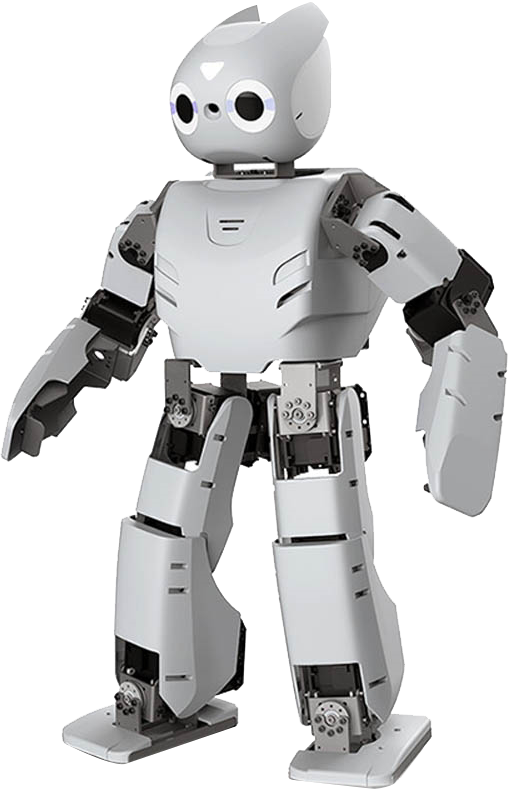
\includegraphics[width=.5\textwidth]{darwin-op-2}
        \end{center}
            
    \end{columns}
  
%*----------- notes
    \note[item]{Notes can help you to remember important information. Turn on the notes option.}
 \end{frame}
 %-
%----------------------------------------------------SLIDE------------------
 \begin{frame}[t, allowframebreaks]{References}
 %\frametitle{References}
%\begin{frame}{Reference}
    %\transboxin[duration=1,direction=30]

    % \begin{bibunit}[plain]
    % \cite{guangyi2018research}.
    % %\cite{kanakia2012}
    % %\cite{agostini2007}
    % %\cite{azuma1997survey}
    % \cite{Buss2005}
  
    % \putbib
    % \end{bibunit}
  
    %\bibliographystyle{IEEEtran}
    %\bibliographystyle{IEEEtranS}
    %\bibliographystyle{IEEEbib}
    \bibliographystyle{abntex2-alf}
    %\bibliographystyle{abntex2-num}
    %\bibliographystyle{abnt-alf}
    \bibliography{bibliography} 
    %\putbib

%*----------- notes
    %\note[item]{Notes can help you to remember important information. Turn on the notes option.}
\end{frame}
%
%-
%*----------- SLIDE-BACKUP ------------------------------------------------------
% \backupbegin
% %
% \begin{frame}{Backup}
%     Test
% %*----------- notes-------------------------------
% \note{Notes can help you to remember important information. Turn on the notes option.}
% \end{frame}
% %-
% \backupend
% %-
%*----------- QUESTIONS ---------------------------------------------------------
\begin{frame}[c,plain]
    \lastpage{
        \begin{center}   
            {\usebeamerfont{title} Questions?}\\[3ex] 
            %\hspace{1.5cm} 
            marco.a.reis@google.com
        \end{center}
    }
    
%*----------- notes---------------------------------
    \note[item]{Notes can help you to remember important information. Turn on the notes option.}
\end{frame}
%*-------------------------------------------------------------------------------
\end{document}